\chapter{Análisis de requisitos}
\label{chap:requisitos}
\section{Funcionalidades}
Esta aplicación dispoñerá de dúas funcionalidades principais:
\begin{itemize}
    \item \textbf{Modo \textit{singleplayer}}: Esta funcionalidade consistirá en permitir ao usuario poder xogar de maneira individual. Neste caso, a aplicación escollerá unha palabra aleatoria dende un dicionario (podendo ser este ampliable polos usuarios) situado nos propios arquivos da aplicación e presentaralla ao usuario por pantalla para que trate de adiviñala.
    \item \textbf{Modo \textit{multiplayer}}: Nesta funcionalidade permitirase xogar a dous ou máis usuarios enfrentándose todos contra todos agrupados en diferentes equipos (que poden ser individuais). O funcionamento segue o mesmo modo que o de \textit{singleplayer} pero cunha ventana na que haxa que tocar a pantalla e que agoche o progreso de cada equipo entre cada turno para evitar trampas. Neste modo de xogo tamén se ofrecerá unha interface na que se declaren os equipos co seu nome (non se levará a cabo a función de rexistro de xogadores xa que non se considera relevante). Por outro lado modo online basearase nun enfrontamento 1 contra 1 como gañador ao xogador que adiviñe a palabra en menos intentos.
\end{itemize}

A prioridade de implementación das funcionalidades seguirá a orde descrita anteriormente, sendo o modo \textit{singleplayer} a primeira funcionalidade en ser implementada, o modo (\textit{multiplayer}) o segundo. \\

Antes destas funcionalidades principais realizaranse funcionalidades a un nivel máis baixo como o menú principal ou o diccionario, que serán as primeiras en ser desenvoltas. \\
\begin{center}
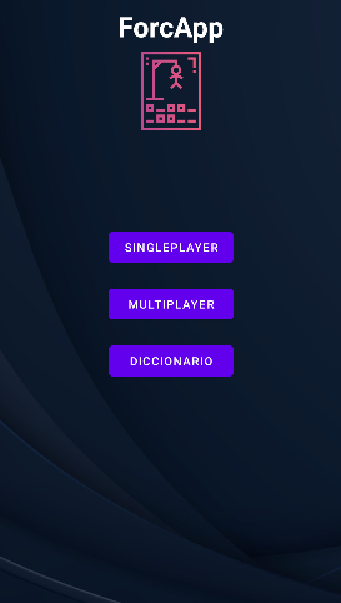
\includegraphics[scale=0.53]{imaxes/menu.png}
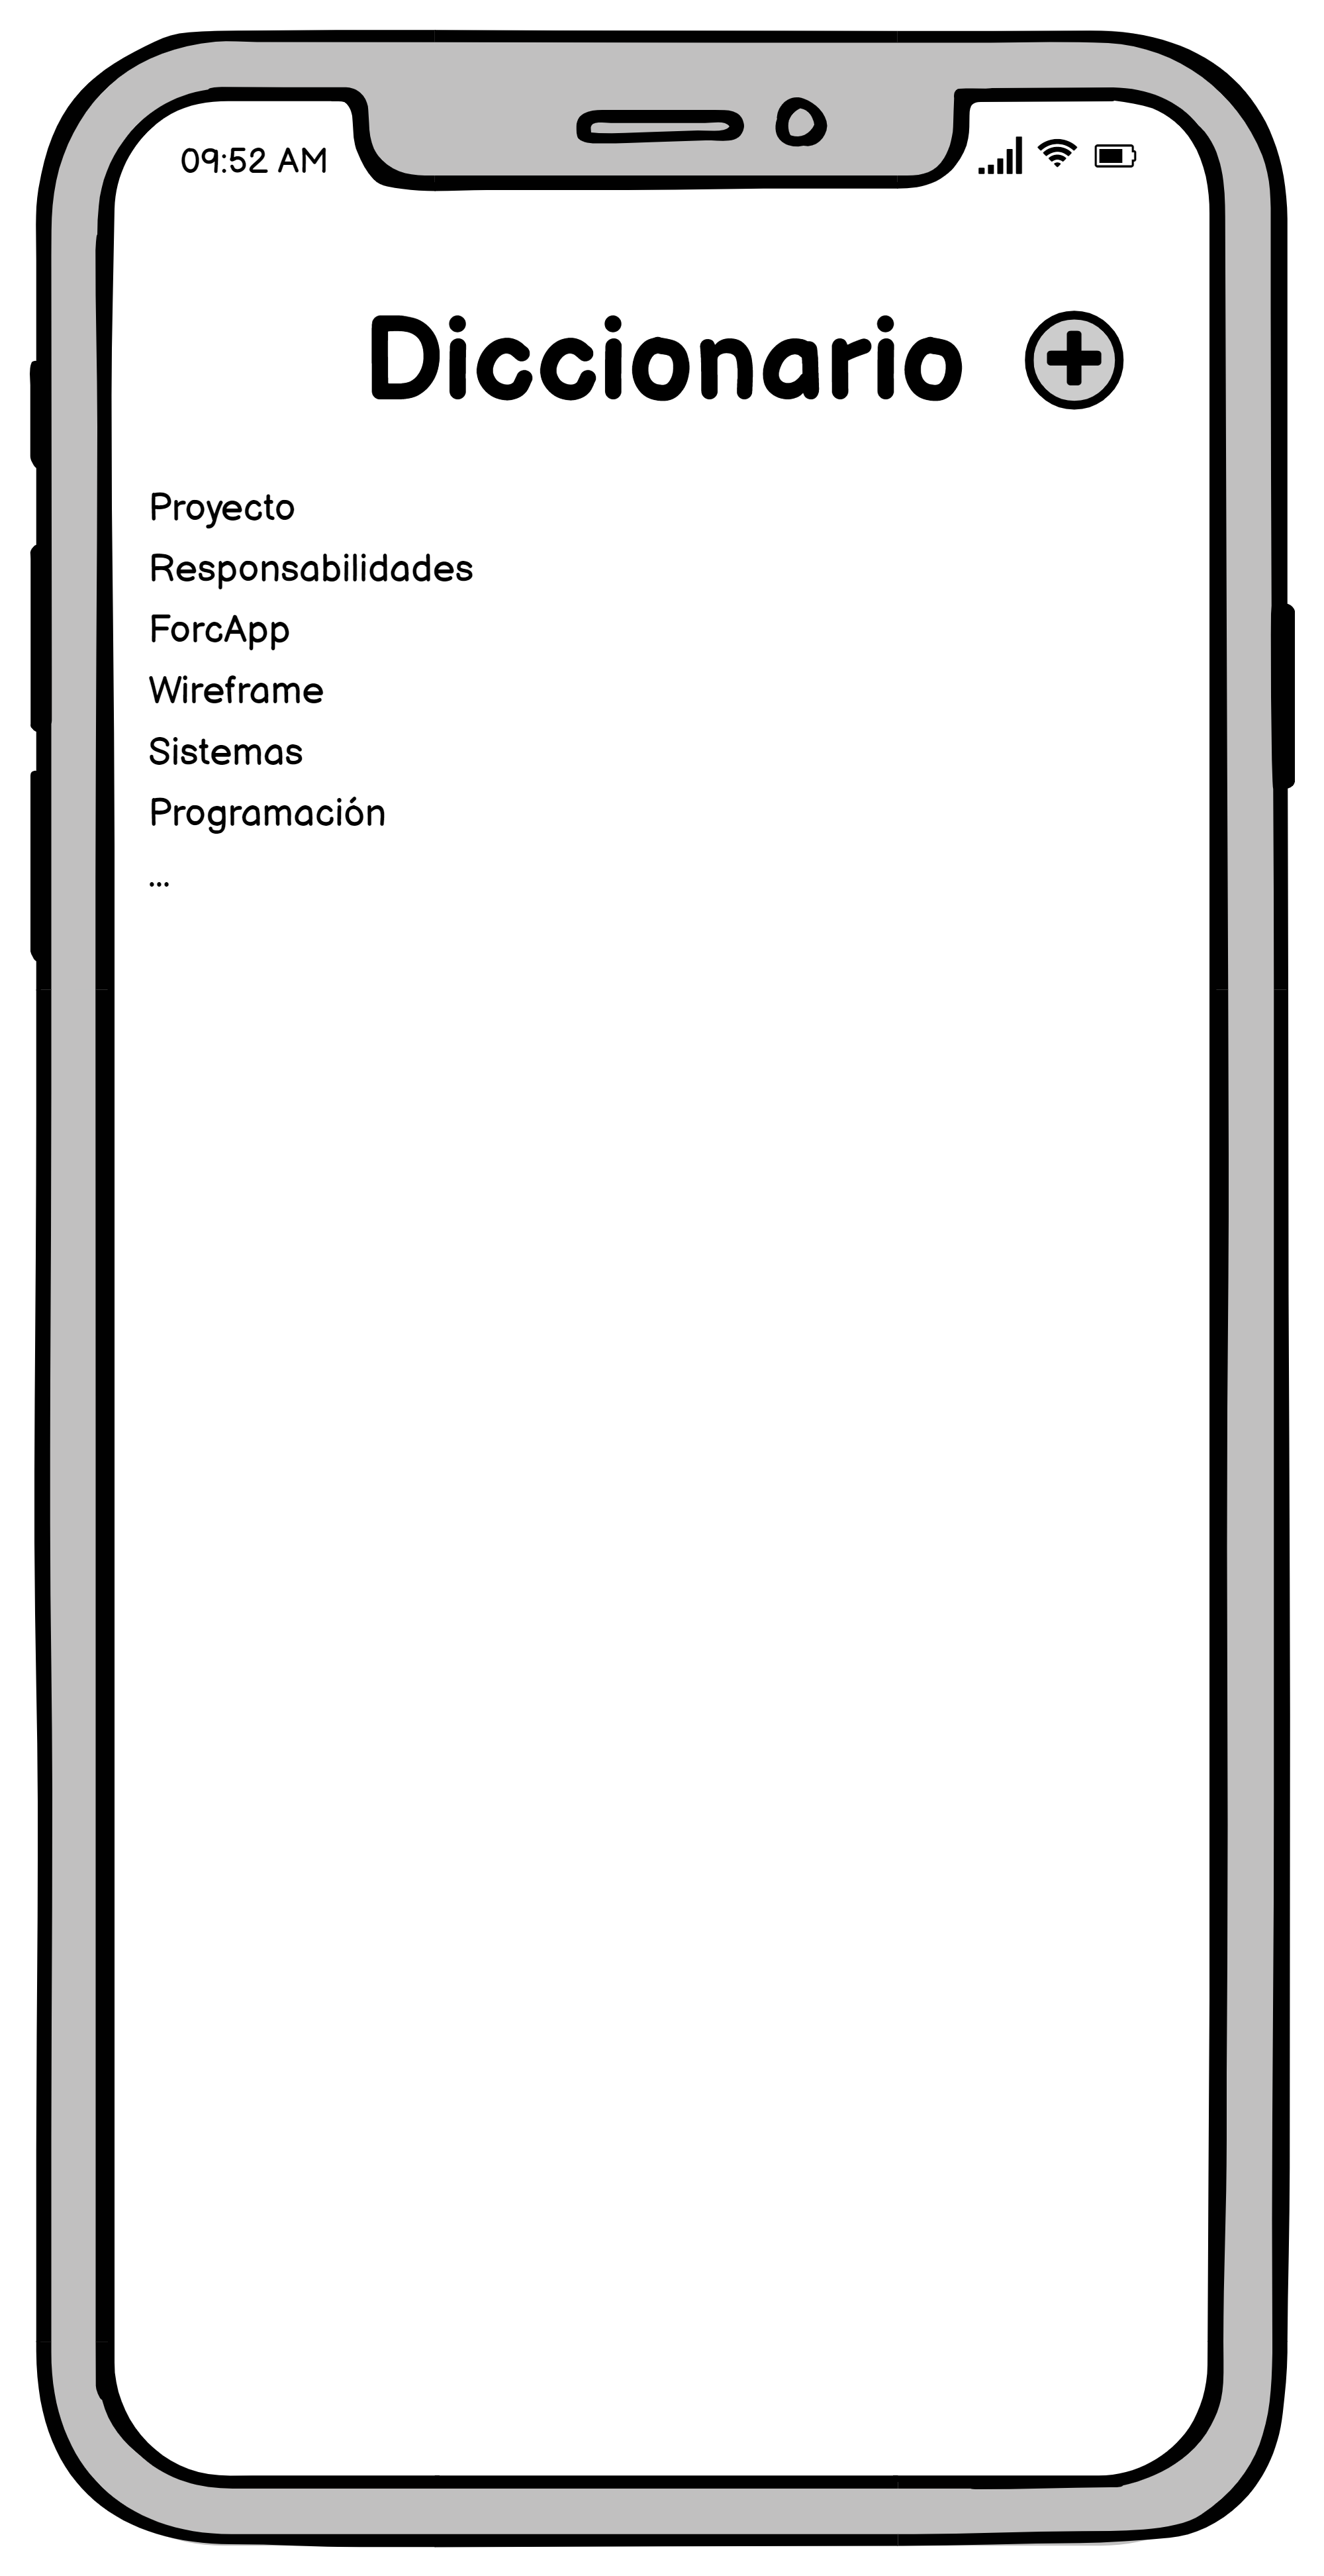
\includegraphics[scale=0.05]{imaxes/diccionario.png}\\ [30 pt]
\end{center}
En traballos futuros pódense engadir novas funcionalidades como levar a conta de partidas gañadas e perdidas (pódense calcular estatísticas como porcentaxes de éxito ou número de intentos medios para obter unha victoria), tanto no modo \textit{singleplayer} como no \textit{multiplayer}. No primeiro modo, servirá a modo de histórico mentras que no segundo caso, definirá quen é o gañador ao final dun número de rondas.

Ademais a aplicación amosará un teclado 'artificial' sen necesidade de usar un do sistema. Ao seleccionar unha letra dese teclado amosarase sombreada e non será posible volver a seleccionala.
 \let\cleardoublepage=\clearpage 